\documentclass[10pt, onecolumn, draftclsnofoot, letterpaper, compsoc]{IEEEtran}

\usepackage{cite}
\usepackage{float}
\usepackage{hyperref}
%\usepackage{enumitem}
\usepackage{graphicx}

% Macro for the signatures
\newcommand*{\SignatureAndDate}[1]{%
    \par\noindent\makebox[2.5in]{\hrulefill} \hfill\makebox[2.0in]{\hrulefill}%
    \par\noindent\makebox[2.5in][l]{#1}      \hfill\makebox[2.0in][l]{Date}%
}

\renewcommand*\contentsname{Table of Contents} % Rename ToC

\newcommand{\myindent}{\hspace{\oldparindent}}

% Temp title and author
\title{Design Document}
\author{Totality AweSun \\
		Bret~Lorimore, Jacob~Fenger, George~Harder \\
		\textit{\today \\
		CS 461 - Fall 2016}}

\begin{document}

\maketitle

\begin{abstract}

This document describes in detail the design for the various components of the
North American Solar Eclipse 2017 senior capstone project. These components are
described according to the IEEE 1016-2009 standard. There are three high level
components detailed in this document, the Eclipse Image Processor, Eclipse Image
Processor Developer Pipeline, and Eclipse Simulator. The sections of this document are broken
into subsections corresponding to these components as applicable.

\end{abstract}

\vspace{10mm}
\noindent \SignatureAndDate{David Konerding, Project Sponsor}
\vspace{8mm}
\noindent \SignatureAndDate{Bret Lorimore}
\vspace{8mm}
\noindent \SignatureAndDate{George Harder}
\vspace{8mm}
\noindent \SignatureAndDate{Jacob Fenger}

\newpage

\tableofcontents

\newpage

%% Section 1
\section{Design Stakeholders and Their Concerns}

The primary stakeholder in this project is David Konerding of Google.
He is one of the managers of the Eclipse Megamovie project that is sponsoring
this Senior Capstone project. David Konerding's concerns are listed below.

\subsection{Image Processor}

\subsubsection{}

The image process needs to take in an image and identify circles which
correspond to the Sun and Moon in the eclipse so it can be stitched into
a timelapse movie by Eclipse Megamovie engineers.

\subsubsection{}

The mean processing time for an image must be one second.

\subsubsection{}

Images must be processed in no longer than five seconds.

\subsubsection{}

Circles corresponding to the Sun and Moon should be found for each image.

\subsubsection{}

The image processor needs to be able to be called by an image processor developer
pipeline with appropriate input data. \\

\subsection{Image Processor Developer Pipeline}

	\subsubsection{}
	Pipeline must collect images from Google Cloud Storage to be run through the image
	processor processor.

	\subsubsection{}
	Pipeline must invoke image processor with images downloaded from Google Cloud
	Storage.

	\subsubsection{}
	Pipeline must aggregate results of image processor run in user friendly HTML file.

	\subsubsection{}
	HTML file should include all information required to re-create any run of the pipeline,
	i.e. image processor git revision, dataset, pipeline command line parameters.

	\subsubsection{}
	All assets required to display HTML file must be uploaded to Google Cloud Storage.
	All links in generated HTML file must correctly reference these assets. \\

\subsection{Eclipse Simulator}
    \subsubsection{}
    The solar eclipse must be accurately simulated based on
    user entered location information.

    \subsubsection{}
    Users will be able to view the eclipse via a
    draggable slider, clickable time step buttons, and a play functionality.

    \subsubsection{}
    The user interface should be visually appealing, easy to navigate, and align
    with the theme of the larger project's site.

    \subsubsection{}
    Simulator will only support locations within continental
    United States.

    \subsubsection{}
    The simulator must load in less than 500ms given a 1-10
    Mbps internet connection. \\


%% Section 2
\section{Design Viewpoints}

\subsection{Image Processor}

\subsubsection{Speed and Performance}

\textbf{Concerns:} 1.1.2, 1.1.3 \\
\textbf{Elements:} 4.1.2, 4.1.3, 4.1.4, 4.1.5, 4.1.9 \\
\textbf{Analytical Methods:} This view is defined by whether or not we are
achieving desired processing speeds for our eclipse images. \\
\textbf{Viewpoint Source:} George Harder \\

\subsubsection{Accuracy}

\textbf{Concerns:} 1.1.1, 1.1.4 \\
\textbf{Elements:} 4.1.1, 4.1.5, 4.1.9 \\
\textbf{Analytical Methods:} Accurately finding the Sun and the Moon in each
eclipse image is very important as it is pertinent to the construction of the
Eclipse Megamovie. \\
\textbf{Viewpoint Source:} George Harder \\

\subsubsection{Input and Output}

\textbf{Concerns:} 1.1.5 \\
\textbf{Elements:} 4.1.2, 4.1.6, 4.1.7, 4.1.8 \\
\textbf{Analytical Methods:} This view will be evaluating whether or not the
input and output of the image process meet the specifications defined in the
design document. \\
\textbf{Viewpoint Source:} George Harder\\

\subsection{Image Processor Developer Pipeline}
    \subsubsection{Image Collection}
    \textbf{Concerns:} 1.2.1, 1.2.2 \\
    \textbf{Elements:} 4.2.1, 4.2.4, 4.2.5 \\
    \textbf{Analytical Methods:} Developer pipeline must be able to use images
    from a specified Google Cloud Storage bucket. \\
    \textbf{Viewpoint source:} George Harder \\

    \subsubsection{Output Generation}
    \textbf{Concerns:} 1.2.3, 1.2.4 \\
    \textbf{Elements:} 4.2.1, 4.2.2, 4.2.3, 4.2.6, 4.2.7, 4.2.8, 4.2.9 \\
    \textbf{Analytical Methods:} Developer pipeline must produce a well
    formatted and visually appealing output document in HTML that includes
    the information specified in sections 1.2.3 and 1.2.4. \\
    \textbf{Viewpoint source:} George Harder \\

    \subsubsection{Output Uploading and Storage}
    \textbf{Concerns:} 1.2.5 \\
    \textbf{Elements:} 4.2.1, 4.2.4, 4.2.5 \\
    \textbf{Analytical Methods:} Developer pipeline must upload the output
    document to Google Cloud Storage so that is easily viewable by the developer
    and any collaborators and must produce working URL's to all referenced
    assets (i.e. images and the document itself). \\
    \textbf{Viewpoint source:} George Harder \\

\subsection{Eclipse Simulator}
  \subsubsection{Interface}
  \textbf{Concerns:} 1.3.2, 1.3.3 \\
  \textbf{Elements:} 4.3.1, 4.3.2, 4.3.3, 4.3.5, 4.3.8 \\
  \textbf{Analytical Methods:} Interface should be appealing
  to the user as well as being responsive and fast. The look and feel of the user
  interface will be evaluated by the sponsor and deemed complete when it meets their
  desired specifications. \\
  \textbf{Viewpoint source:} Jacob Fenger \\

  \subsubsection{Performance}
  \textbf{Concerns:} 1.3.2, 1.3.5 \\
  \textbf{Elements:} 4.3.4, 4.3.7, 4.3.8,  \\
  \textbf{Analytical Methods:} The initial loading time
  of the simulator should be fast. Additionally, the
  interactions that the user has with the simulator should
  be responsive and should not show any significant slow
  downs. \\
  \textbf{Viewpoint source:} Jacob Fenger \\

  \subsubsection{Simulation Accuracy}
  \textbf{Concerns:} 1.3.1, 1.3.4 \\
  \textbf{Elements:} 4.3.4, 4.3.6 \\
  \textbf{Analytical Methods:} In the simulator, the Sun and
  Moon display should reflect scientific accuracy when it
  comes to relative position and sizes. Additionally, the
  view of the Sun and Moon above the horizon shall be
  accurate.\\
  \textbf{Viewpoint source:} Jacob Fenger \\


%% Section 3
\section{Design Views}

\subsection{Image Processor}

\subsubsection{Speed and Performance [Governed by Viewpoint 2.1.1]}

The Eclipse Megamovie project expects to receive photographs on the order of
hundreds of thousands from the numerous citizen photographers registered with
the project. This being the case, it is of utmost importance that the image
processor we are building for the project can process images in a timely manner.
This is not only important to being able to build a movie from the images soon
after the eclipse, but also because it prevents storage spaces on either end of
the image processing pipeline from becoming clogged.

In order to achieve these design goals, we are designing a system that uses the
OpenCV C++ library.  This API provides us with high performing library methods,
like Hough transforms, image crops, and image rotations that are necessary to
the image processor's core functionality. In addition to the use of this
language and library, we are making it very easy for anyone to inherit from
the base processing class so one can manipulate specific parts of the
processing pipeline. The interface we are using for the input and output of
the processing easily allows another application, such as the image processor
developer pipeline, to build and run it. \\

\subsubsection{Accuracy [Governed by Viewpoint 2.1.2]}

From a high level, the most fundamental concern in the design of the image
processor is that it can accurately identify the Sun and/or Moon in an eclipse
image. The other concerns associated with the design of the image processor
are near meaningless if the application is not capable of identifying circles
that correspond to the Sun and/or Moon.

To address this concern, we are designing this application with accuracy as a
primary goal. To meet this goal, the system will build upon an existing
eclipse identification algorithm. This algorithm, with improvements we add
ourselves, will be the basis for the parts of the system that we design to
meet the accuracy requirements of the image processor.\\

\subsubsection{Input and Output [Governed by Viewpoint 2.1.3]}

The image processor is one component in a much larger system. For the system to
function the image processor needs to interface with the other components in a
well defined and seamless manner. In addition to speed and accuracy, we need to
design the system with a view toward optimizing the way the image processor
interacts with other components.

To ensure a smooth interface with the image processor developer pipeline we
are designing the image processor to accept a well defined set of command line
arguments including a list of images containing their paths to be processed,
the running mode (Window or batch), the path to an output directory (If ran in
batch mode), and other optional paramaters involving the cv::HoughCircles
function call. The design of the image processor also takes into account the
needs of the engineers handling the processed images. The image processor will
write processed images and their metadata in a specific format to the
specified output directory. \\

\subsection{Image Processor Development Pipeline}

    \subsubsection{Image Collection [Governed by viewpoint 2.2.1]}
    The image processor developer pipeline seeks to provide developers with an
    easy to use interface to the image processor. As such, it is integral to the
    design of the system that it can interface with Google Cloud Storage and
    thereby provide the developer with access to any bucket of test images. In
    order to provide this functionality to developers the image processor
    developer pipeline will accept as an argument the name of a Google Cloud
    Storage bucket. The pipeline will then download the images in this bucket
    and run the image processor over the downloaded images. This streamlines the
    process of testing the image processor and gives developers fine grained but
    simple control over runs of the image processor.  \\

    \subsubsection{Output Generation [Governed by viewpoint 2.2.2]}
    The image processor developer pipeline shall produce an easily readable and
    well formatted HTML document that details information about the run and the
    run itself. For this system to be effective we need to give developer the
    ability to easily reproduce runs and then compare the results of these
    runs. With this in mind, we are designing the output generation portion of
    the pipeline to parse the result of the image processor, which are in a text
    file, and display them, along with metadata like a timestamp, git hash, and
    scoring metrics in an HTML document so that a developer can quickly diagnose
    what impact their changes to the processor had on the results. \\

    \subsubsection{Output Uploading and Storage [Governed by viewpoint 2.2.3]}
    Our image processor developer pipeline must not only produce useful output
    but in addition store that output in a convenient location. To fulfill this
    goal the image processor developer pipeline will upload its output to
    Google Cloud Storage and produce a working URL to the output. This way, a
    developer can share the results of a run with collaborators. Designing the
    image processor pipeline in this way further facilitates continued
    development of the image processor. \\

\subsection{Eclipse Simulator}

  \subsubsection{User Interface View [Governed by Viewpoint 2.3.1 ]}
  The user interface shall utilize 2D animated depictions of
  the Sun and the Moon positioned based on the time and location the simulator
  is set to. In addition to the Sun and Moon, the user interface will contain
  stylized background imagery of a hillside. The simulator's controls will be
  split into a top bar and bottom bar. The top bar will have a location entry
  box, an expandable map, and a zoom button. The bottom bar will have a time
  slider, time up and down buttons, a play/pause button, and a menu to select
  the play speed.  \\

  \subsubsection{Operating Performance View [Governed by Viewpoint 2.3.2]}
  The simulator will have low loading times to ensure smooth performance
  for most users. The simulator will be responsive and quickly respond to
  user input. \\

  \subsubsection{Eclipse Accuracy View [Governed by Viewpoint 2.3.3]}
  The simulator shall display an accurate dipiction of the eclipse from
  any location in the continental United States. This accuracy includes
  accurate relative Moon and Sun sizes, positions in the rendered scene,
  and positions relative to one another. This accuracy shall be evaluated
  by our client and will be marked as adaquate when it meets their expectations. \\

%% Section 4
\section{Design Elements}

\subsection{Image Processor}

\subsubsection{OpenCV}
\textbf{Type:} Library\\
\textbf{Purpose:} OpenCV is the computer vision library we will use to process
images. This open source library can quickly crop and otherwise manipulate
images. It best suits our needs for a computer vision utility.\\

\subsubsection{C++}
\textbf{Type:} Class\\
\textbf{Purpose:} This application will be written in C++ in order to give us
better control over the speed at which the application runs and the necessary
functionality for reading and writing files. \\

\subsubsection{Image Processing Time}
\textbf{Type:} Constraint\\
\textbf{Purpose:} This element exists because our requirements specify that the
average time for an image to be processed must be less than one second.\\

\subsubsection{Serial Image Processing}
\textbf{Type:} Framework\\
\textbf{Purpose:} The image processor will process images one at a time. \\

\subsubsection{Hough Transform}
\textbf{Type:} Procedure\\
\textbf{Purpose:} The Hough transform is an algorithm for identifying circles
and lines in images. It will be used by the image processor to identify total
eclipse images. OpenCV has the circular Hough transform built in. \\

\subsubsection{Command Line Arguments}
\textbf{Type:} Constraint\\
\textbf{Purpose:} The image processor needs to have a well defined set of
command line arguments so that it can interface with the image processor
developer pipeline without difficulty. \\

\subsubsection{Data writer}
\textbf{Type:} System\\
\textbf{Purpose:} This component is meant to encapsulate the functionality
necessary to write the processed images and their associated metadata to an
output directory.\\

\subsubsection{Image Data Structure}
\textbf{Type:} Class\\
\textbf{Purpose:} This class will encapsulate the information and methods needed to manage the images we will be processing. It will also work closely with the Data Writer to write images and their metadata to files.\\

\subsubsection{Solar Eclipse Image Standardisation and Sequencing (SEISS)}
\textbf{Type:} Procedure\\
\textbf{Purpose:} The SEISS algorithm is an image processing algorithm that can
identify images of eclipses, including eclipses at totality \cite{imgKrista}.
We will be basing part of the image processor off of this algorithm. \\

\subsection{Image Processor Development Pipeline}

    \subsubsection{Bash Script}
    \textbf{Type:} System \\
    \textbf{Purpose:} The image processor developer pipeline will consist, in
    part, as a Bash script that handles upload, download, calling the processor,
    and calling the output generator. \\

    \subsubsection{Python}
    \textbf{Type:} Class \\
    \textbf{Purpose:} In order to parse output of the image processor and
    produce an HTML document the image processor developer pipeline will call a
    Python script that handles this functionality. \\

    \subsubsection{Jinja 2}
    \textbf{Type:} Library \\
    \textbf{Purpose:} Jinja 2 is an HTML templating library for the Python
    language. We will use it in our output generation script to fill the HTML
    document with information and results from the run. \\

    \subsubsection{Google Cloud Storage}
    \textbf{Type:} System \\
    \textbf{Purpose:} Google Cloud Storage is a system that we will use to store
    test image datasets and the results of runs of the image processor. \\

    \subsubsection{GSUtil}
    \textbf{Type:} System \\
    \textbf{Purpose:} GSUtil is a command line application that handles
    interaction with Google Cloud Storage. We will use it in our Bash Script as
    an interface to Google Cloud Storage for image download and output upload. \\

    \subsubsection{HyperText Markup Language (HTML)}
    \textbf{Type:} System \\
    \textbf{Purpose:} HTML is a language for formatting and aranging data. We
    will use it to format the results of a run of the image processor. \\

    \subsubsection{Javascript}
    \textbf{Type:} System \\
    \textbf{Purpose:} Javascript provides functionality to HTML documents, we
    will use it to handle sorting of the rows in the table that holds the
    output in the output HTML document. \\

    \subsubsection{Cascading Style Sheets (CSS)}
    \textbf{Type:} System \\
    \textbf{Purpose:} CSS handles the styling, look, and feel of HTML documents.
    In our context, it is used to make the output HTML document visually
    appealing and easy to read. \\

    \subsubsection{Material Design Lite (MDL)}
    \textbf{Type:} Library/Framework \\
    \textbf{Purpose:} MDL is a framework that provides built in CSS for HTML
    elements like text, lists and tables. We will use it to enhance the CSS on
    our page and make the data easily readable and visually appealing. \\


\subsection{Eclipse Simulator}

  \subsubsection{Hypertext Markup Language (HTML)}
  \textbf{Type:} System \\
  \textbf{Purpose:} HTML will be used to describe the basic
  view structure of the simulator. \\

  \subsubsection{Cascading Style Sheets (CSS)}
  \textbf{Type:} System \\
  \textbf{Purpose:} CSS will be used to style the simulator
  HTML. This includes layout, color, shape, fonts,
  and more. \\

  \subsubsection{Scalar Vector Graphics (SVG)}
  \textbf{Type:} System \\
  \textbf{Purpose:} This element will be used to
  position the Sun/Moon within the simulator scene. \\

  \subsubsection{MeuusJS JavaScript Library}
  \textbf{Type:} Library \\
  \textbf{Purpose:} This library is used to compute the position
  of the Sun and Moon in the sky at a given time/position. \\

  \subsubsection{View}
  \textbf{Type:} Component \\
  \textbf{Purpose:} The simulator view will be responsible
  for managing any dynamic components of the simulator front end.
  This includes manipulating the HTML DOM, updating styles, and updating SVG
  elements. \\

  \subsubsection{Model}
  \textbf{Type:} Component \\
  \textbf{Purpose:} The model will perform complex computational tasks in the simulator.
  This will include providing a wrapper around the MeuusJS library, and implementing
  other computations based on the information returned by this library. \\

  \subsubsection{Controller}
  \textbf{Type:} Component \\
  \textbf{Purpose:} The controller will coordinate interaction between the view and
  the model. The controller will also provide the entrypoint for the simulator. \\

  \subsubsection{Model-View-Controller Architecture}
  \textbf{Type:} Relationship \\
  \textbf{Purpose:} This architecture is defined by the interactions of the model,
  view, and controller entities. \\

%% Section 5
\section{Design Overlays}

\subsection{Image Processor}

\begin{figure}[H]
    \centering
    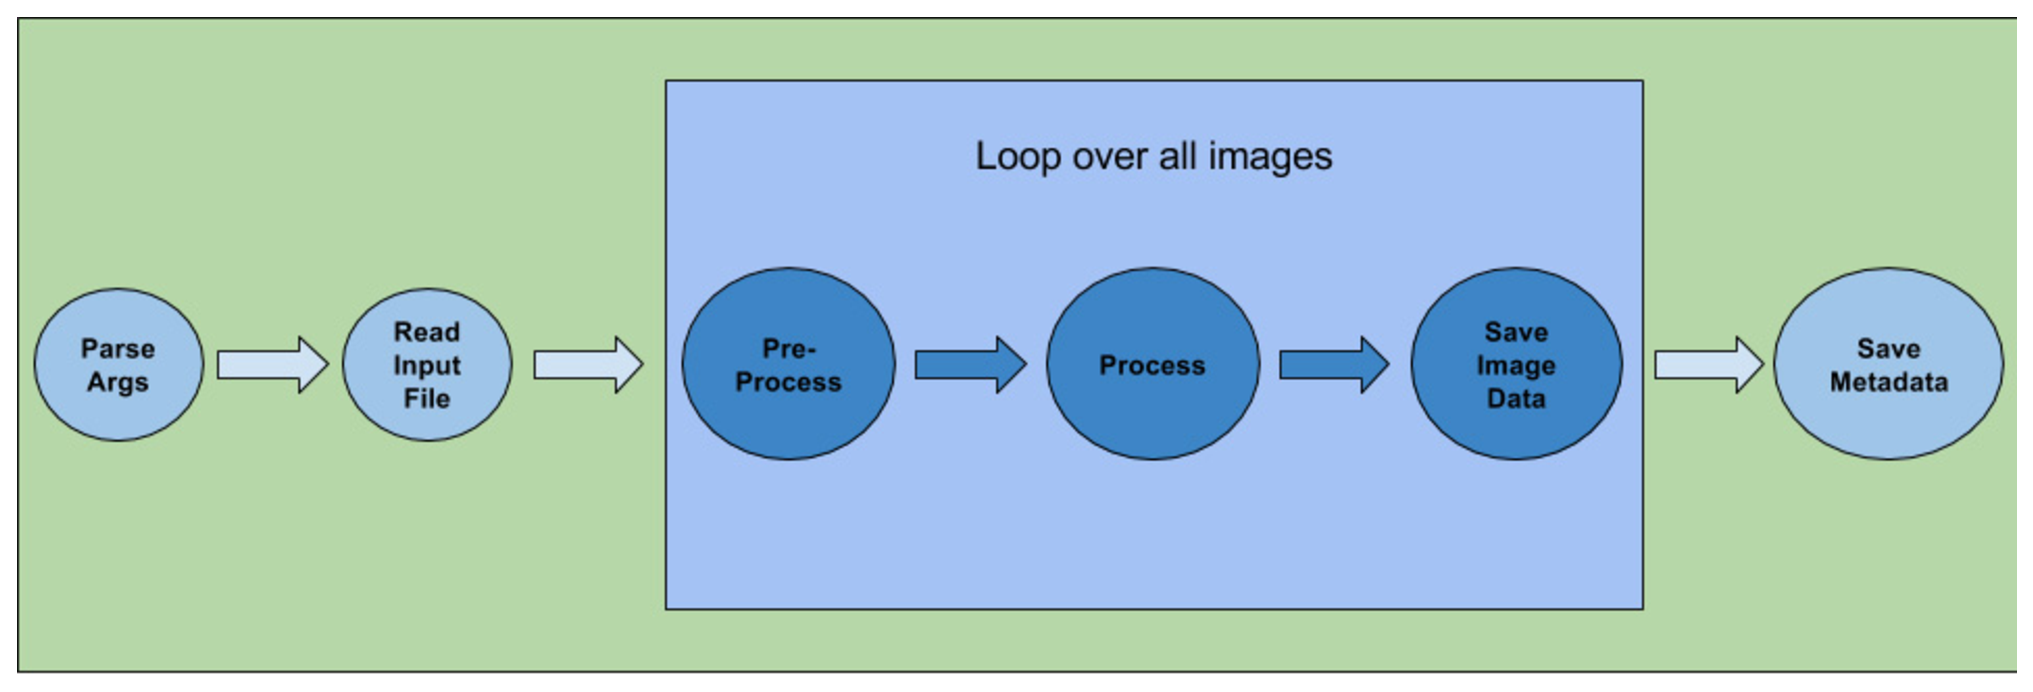
\includegraphics[width=\textwidth]{imgproc.eps}
    \caption{Image processor basic dataflow}
\end{figure}

\subsection{Image Processor Developer Pipeline}

\begin{figure}[H]
    \centering
    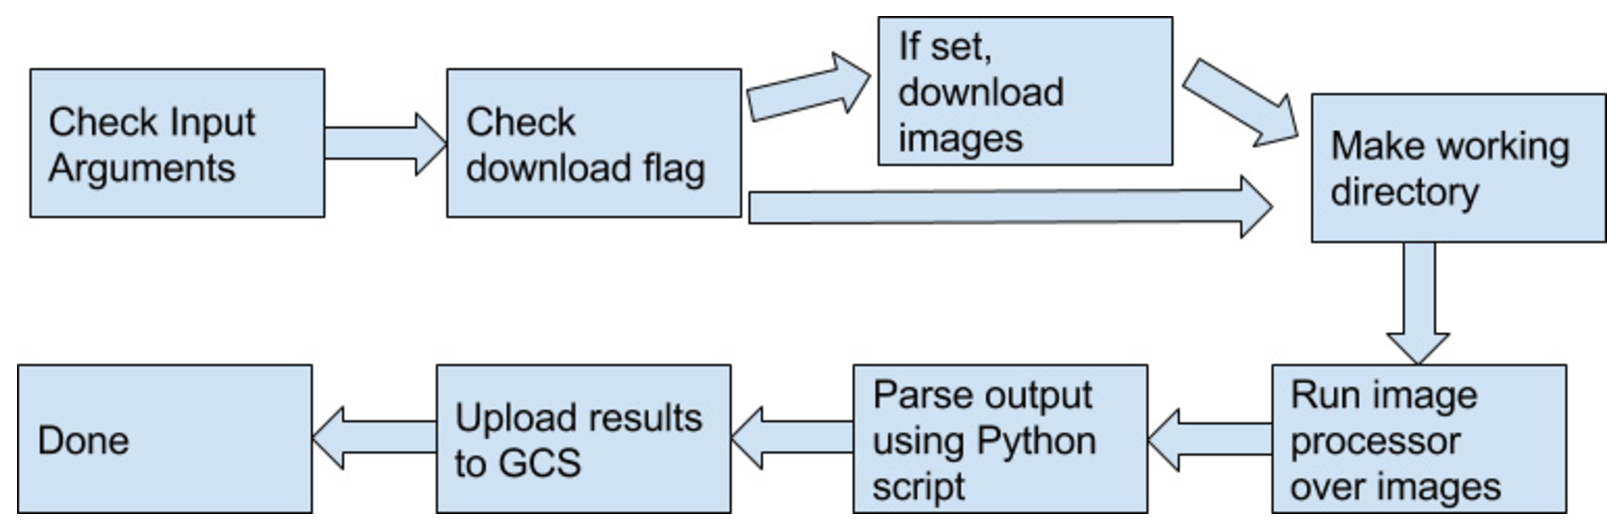
\includegraphics[width=0.75\textwidth]{dev.eps}
    \caption{Image processor developer pipeline basic dataflow}
\end{figure}

\subsection{Eclipse Simulator}

\begin{figure}[H]
    \centering
    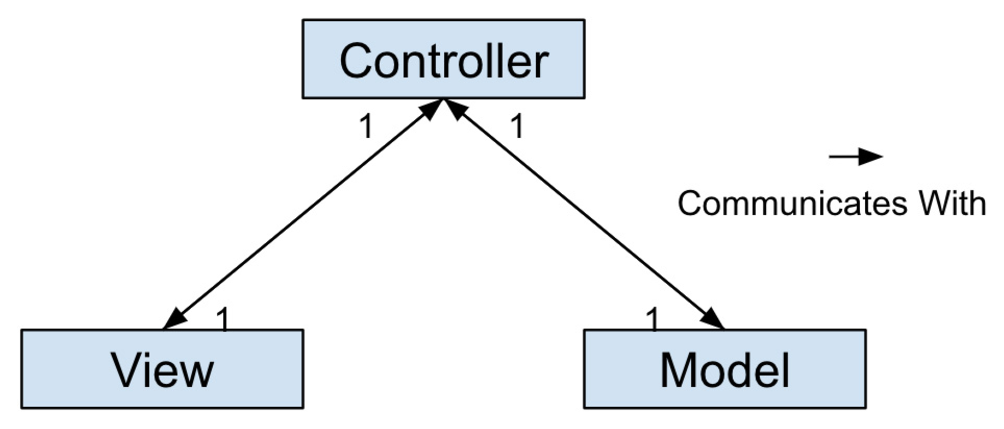
\includegraphics[width=0.5\textwidth]{jake_fig.eps}
    \caption{Eclipse simulator MVC architecture}
\end{figure}


%% Section 6
\section{Design Rationale}

\subsection{Image Processor}

The design of this system is based on needs surrounding accuracy, speed, and
ability to interface with other components in the larger system. As was detailed
in the technology review, we made certain decisions about what tools and
algorithms to use based on the specific requirements of our system. The use of
these tools has necessarily shaped the design of this application.

Additional information regarding design rationale can be found in the 'Purpose'
section of the design elements. \\

\subsection{Image Processor Developer Pipeline}

We chose to compose the various compose the various elements of the developer using
a bash script for several reasons. First, it allowed us to use the gsutil command
line utility to download/upload images from Google Cloud Storage. This was desirable
as gsutil already implements error handling, authentication, and concurrent downloads,
meaning that these were not things we had to worry about implementing. Using bash also
allowed us to build the latest version of the image processor using make, and to
then easily invoke it with the input images. Bash also allowed us to use command line
utilities like find, grep, and cut to dynamically create a input images file for the image
processor without having to write any code. \\

\subsection{Eclipse Simulator}

The goals for the simulator were to provide a fast and
responsive experience to the user while providing
scientifically accurate results. The simulator is a rather
complex application. One of our main goals was to design it
such that iterative development was streamlined.

We decided to utilize the MVC architecture to allow for increased
separation of application logic. In the technology review,
we compared two libraries: Suncalc and Ephemeris. Initially, we chose
SunCalc as the better library due to better documentation and ease of use. After
further testing, we determined that the results of both of these libraries were
unsatisfactorily accurate and opted for another choice: MeuusJS. The Meuus library
provides us with Sun/Moon positions that meet the requirements for accuracy of
this simulator. The separation of application logic afforded by the MVC architecture
means that switching between these libraries would be very easy and touch only a very
small portion of the codebase.

We chose to utilize SVG for the Sun/Moon positioning as it implements a simply x, y
coordinate system and is very fast. \\

%% Section 7
\section{Design Languages}

\begin{enumerate}
    \item \href{http://www.omg.org/spec/UML/2.5}{UML Version 2.5}
\end{enumerate}

%% Supporting Info

\newpage
\section{Appendices}

\subsection{Appendix I: Change History}

\begin{enumerate}
\item November 30th, 2016 -- Document Created
\item May 15th, 2017 -- Document revised based on updated requirements \\
\end{enumerate}

\subsection{Appendix II: Glossary of Terms}

\textbf{Eclipse Megamovie Project:}
The Eclipse Megamovie Project is a collaboration between Google
and scientists from Berkeley and several other institutions with the
aim of collecting large quantities of observations of the solar eclipse
that will pass over the United States on August 21, 2017. The project
will crowdsource photos of the eclipse from photographers at various
points along the path of totality. \\

\noindent \textbf{VM:}  A virtual machine - a hosted virtual server. In this
document, when we refer to a VM we are specifically referring to a VM hosted in
Google Cloud - this could be either a bare VM or a single node in a VM cluster.\\

\noindent \textbf{Google Cloud Storage:}  A fully managed file storage solution
offered from Google, optimized for storing/accessing large files.\\

\noindent \textbf{Mbps:} Megabits per second. This is referring to download and
upload speeds.\\

\noindent \textbf{Ephemeris:} An ephemeris is used to give positional information
about astronomical objects. We are using a JavaScript library, meuus.js, as our
ephemeris.\\

\noindent \textbf{Machine:} The term machine is used throughout this document in
reference to a particular VM instance.\\

\noindent \textbf{JPEG/JPG:}
JPEG is a lossy compression technique for images. When we refer
to JPEG/JPG files in this document we are referring to image files
compressed in this method with the .jpeg or .jpg file extension. \\

\noindent \textbf{PNG:}
PNG refers to the Portable Network Graphics image file format.
Images in the PNG format are frequently referred to as "PNGs" and are
saved with the .png file extension. \\

\noindent \textbf{SEISS:} Solar Eclipse Image Standardisation and Sequencing.
This refers to an algorithm developed by Krista et al. \cite{imgKrista} that
seeks to identify eclipse images and classify them by the phase that the
eclipse is in. We will be using and modifying this algorithm to suit the needs
of this project. \\

\bibliographystyle{IEEEtran}
\bibliography{des-doc}

\end{document}

